\section{Hybrid Control System Model}
Insert introduction text here

\subsection{Hybrid Control Systems}
Insert introduction text here.
\begin{figure}[t!]
\centering
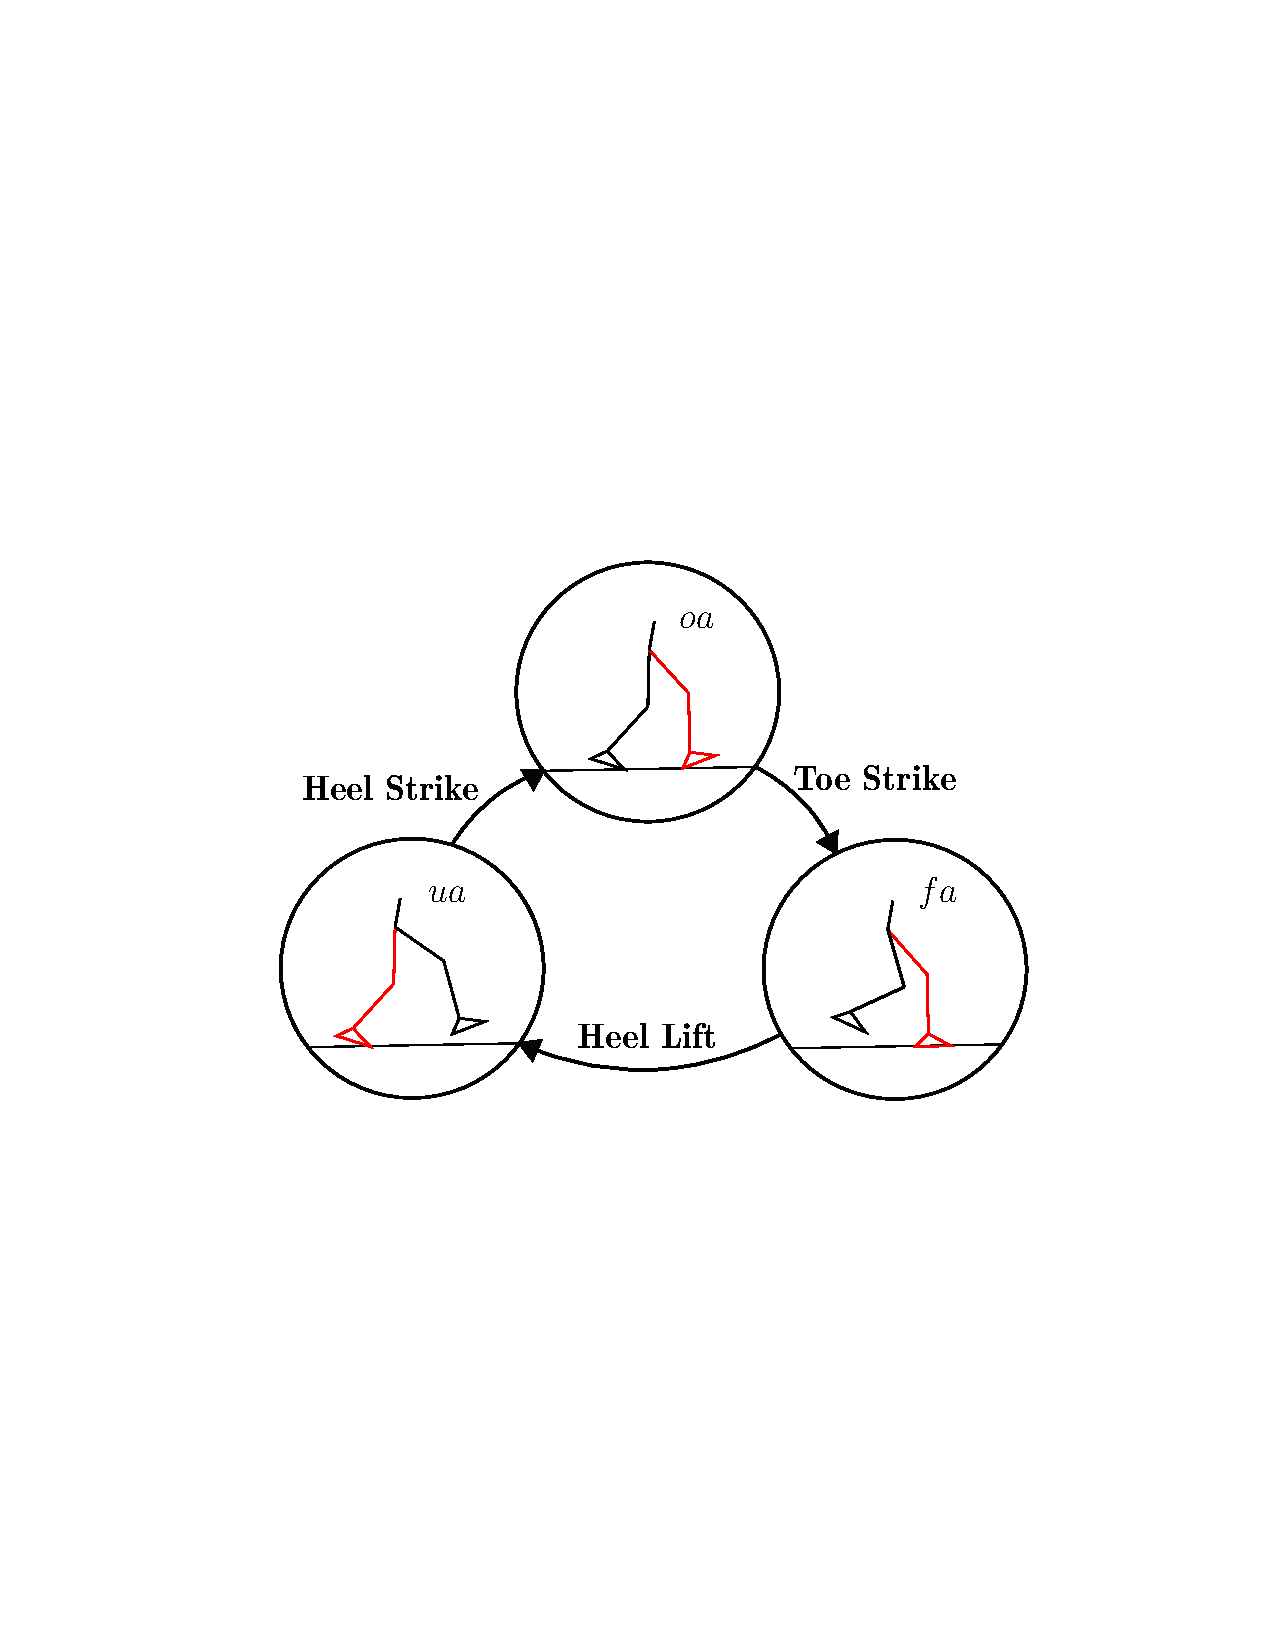
\includegraphics[width=0.45\textwidth]{figures/DomainGraph.pdf}
\caption{Ordering of the domain structure for 3-domain walking. }
\label{fig:DomainGraph}
\end{figure}

\newsec{Graphs and Cycles.} A graph is a tuple $\Graph = (\VertexSet, \EdgeSet)$, where $\VertexSet$ is the set of vertices and $\EdgeSet \subset \VertexSet \times \VertexSet$ is the set of edges; an edge $\edge \in \EdgeSet$ can be written as $\edge = (i,j)$, and the source of $\edge$ is $\sore = i$ and the target of $\edge$ is $\tare=j$. Here, we are interested in hybrid systems \textit{on a cycle}; therefore, we are interested in graphs that contain cycles or are themselves cycles. A \textit{directed cycle} (or just a cycle) is a graph $\cycle = (\VertexSet, \EdgeSet)$ containing  $b \in \Integers$ edges and vertices that can be written as:

\begin{align}
 \VertexSet &= \{ \vertex_0,\vertex_1, \ldots ,\vertex_{b-1}\}\\
 \EdgeSet   &= \{ \edge_0 = (\vertex_0,\vertex_1), \ldots ,\edge_{b-1}=(\vertex_{b-1},\vertex_0)\}.\nonumber
\end{align}

Since in the case of a cycle, the edges are completely determined by the vertices, we sometimes simply denote a cycle by: $\cycle : \vertex_0 \to \vertex_1 \to \cdots \to \vertex_{b-1} \to \vertex_b = \vertex_0$. In the case when a graph $\Graph$ is being considered with more than one cycle, we denote a cycle in the graph by $\cycle \subset \Graph$.

\begin{myexample}
 The domain graph pictured in FIGREF has an underlying graph that is a directed cycle: $\Graph_w = (\VertexSet_w,\EdgeSet_w)$. In particular, there are 3 vertices and edges, which results in the cycle:
 \begin{align}
    \cycle_w &:  \underbrace{[st,nst]}_{ds} \to  \underbrace{[st,sh]}_{fa} \to  \underbrace{[st]}_{ua} \to  \underbrace{[st,nst]}_{ds}
 \end{align}
 where $ds$, $fa$ and $ua$ are labels for the three vertices: double support, single-support with full actuation and single-support with underactuation.
\end{myexample}

With the notion of a directed cycle, we can introduce the formulation of a hybrid system that is of interest in this paper.
%%%% Standard Hybrid Control System definition
\begin{mydefinition}
 A hybrid control system in a cycle is a tuple
 \begin{align}
  \HC = (\cycle, \domain, \admissiblecontrol, \guard, \resetmap, \controlsystem),
 \end{align}
 where
 \begin{itemize}
  \item $\cycle = (\VertexSet, \EdgeSet)$ is a directed cycle,
  \item $\domain = \{ \indexbyvertex{\domain} \}_{\vertex \in \VertexSet}$ is a set of domains, where $\indexbyvertex{\domain} \subseteq \Reals^{\indexbyvertex{\dimensionx}} \times \Reals^{\indexbyvertex{\dimensionu}}$ is a smooth submanifold of $\Reals^{\indexbyvertex{\dimensionx}} \times \Reals^{\indexbyvertex{\dimensionu}}$ (with $\Reals^{\indexbyvertex{\dimensionu}}$ representing conrol inputs),
  \item $\admissiblecontrol = \{ \indexbyvertex{\admissiblecontrol} \}_{\vertex \in \VertexSet}$, where $\indexbyvertex{\admissiblecontrol} \subset \Reals^{\indexbyvertex{\dimensionu}}$ is a set of admissible controls,
  \item $ \guard = \{ \indexbyedge{ \guard} \}_{\edge \in \EdgeSet}$ is a set of guards, where $\indexbyedge{\guard} \subseteq \indexbysource{\domain}$,
  \item $\resetmap = \{ \indexbyedge{\resetmap} \}_{\edge \in \EdgeSet}$ is a set of reset maps, where $\indexbyedge{\resetmap}: \Reals^{\indexbysource{\dimensionx}} \to \Reals^{\indexbytarget{\dimensionx}}$ is a smooth map,
  \item $\controlsystem = \{ \indexbyvertex{f},\indexbyvertex{g} ) \}_{\vertex \in \VertexSet}$, where $(\indexbyvertex{f}, \indexbyvertex{g})$ is a control system on $\indexbyvertex{\domain}$, i.e. , $\xdot = \indexbyvertex{f}(\x) + \indexbyvertex{g} (\x) \control$ for $\x \in \indexbyvertex{\domain}$ and $\control \in \indexbyvertex{\admissiblecontrol}$.
 \end{itemize}

\end{mydefinition}

\subsection{General Robot Hybird Control System}
This section describes how to construct a hybrid control system for a robot walking on a flat, rigid surface.

\newsec{The Terrain and the Robot.}
Let $R_0$ be a fixed inertial or world-frame. Denote the three orthonormal axes of the world frame $R_0$ by $({\hat x}, {\hat y}, {\hat z})$ and without loss of generality, orient $R_0$ such that ${\hat z}$ is aligned parallel to gravity, e.g. ${\hat z}$ points up. Let $\mathbf{p^0}$ $ = (p^x,p^y,p^z)^T \in \Reals^3$ denote a \textit{point} expressed in the world frame. Let $\Terrain$ be a fixed rigid body, called the \textit{terrain} with a surface defined by the plane $\Terrain = \{(p^x,p^y,p^z)_0 \in \Reals^3 : p^z = 0\}$; the terrain represents a perfectly flat walking surface.

Let the biped model of interest be a collection of rigid links--each with finite length and mass--together with a collection of revolute joints. Let $R_b$ be a reference frame attached to the body of the biped with position $\mathbf{p_b}$ $ \in \Reals^3$ and orientation $\mathbf{\phi_b}$ $ \in SO(3)$. Consider a configuration space for the biped $\indexbyrobot{\ConfigurationSpace}$, i.e. a choice of (body or shape) coordinates for the robot where typically $\indexbyrobot{\q} \in \indexbyrobot{\ConfigurationSpace}$ is a collection of (relative) joint angles; i.e. angles between successive links of the robot. The \textit{generalized coordinates} of the robot are then given by $\q = (\mathbf{p_b}^T, \mathbf{\phi_b}^T, \indexbyrobot{\q}^T)^T \in \ConfigurationSpace = \Reals^3 \times SO(3) \times \indexbyrobot{\ConfigurationSpace}$, with $\ConfigurationSpace$ the generalized configuration space.

Let $P_r$ denote the uncountably infinite set of all positions on the biped expressed in $R_0$. Each position of the robot in the world frame $\mathbf{p_i} \in P_r$ can be expressed as a function of the generalized coordinates $\q$; that is, $\mathbf{p_i} = {\hat f}(\q)$ for a forward kinematics map ${\hat f}: \Reals^3 \times SO(3) \times \indexbyrobot{\ConfigurationSpace} \to \Reals^3$, or in other words, use geometry to compute positions on the robot as functions of $\q$.

\begin{myexample}
 The robot of interest in this work is a model of the Texas A\&M University AMBER Lab's robot: AMBER 2 (successor to AMBER 1), shown in Fig. \ref{fig:robot}. The configuration space of AMBER 2, $\indexbyrobot{\ConfigurationSpace}$, is given by the coordinates $\indexbyrobot{\q} = \{ \qsa, \qsk, \qsh, \qnsh, \qnsk, \qnsa\}$. The inertial and length properties of AMBER 2 are given in Table \ref{table:params}, near the end of the paper.
\end{myexample}


\newsec{Robot Dynamics.}
The Lagrangian of a bipedal robot, $\Lagrangian : TQ \to \Reals$, can be stated in terms of kinetic and potential energies as:
\begin{align}
 \nonumber
 \Lagrangian(\q,\dq) = \KineticEnergy(\q,\dq) - \PotentialEnergy(\q).
\end{align}
The Euler-Lagrange equations yield the equations of motion, which for robotic systems REFERENCE are stated as follows:
\begin{align}
 \GeneralizedInertia\ddq + \CoriolisGravity = \TorqueDistribution \control,
 \label{eq_eulerlagrange}
\end{align}
where $\GeneralizedInertia$ is the generalized inertia matrix, $\CoriolisGravity = \Coriolis + \Gravity$ contains the Coriolis and gravity effects, $\TorqueDistribution$ is the torque distribution matrix, $\control$ is the vector of actuator torques.

\newsec{Robot-Terrain Interaction/Contacts.} In locomotion, the robot leverages interactions with the terrain to accelerate its links and thus form a \textit{gait}. In periodic locomotion, the robot-terrain interactions occur in a small subset of points on the robot--termed \textit{contact points}. Specifically, the \textit{set of contact points} is the set $\ContactSet = \{ \contact_1, \contact_2, \ldots, \contact_\dimensioncontacts\}$, where each $\contact_i$ is an identifier of a specific location on the biped which will eventually contact the ground in a given gait.

\begin{myexample}
 The set of contact points for AMBER2 during a three-domain cycle, as illuminated on the robot in Fig. \ref{fig:DomainGraph}, is $\ContactSet = \{sh, st, nsh, nst \}$, where $sh$ and $st$ indicate the stance left heel and toe, and $nsh$ and $nst$ indicate the nonstance heel and toe, respectively. Here, the terms stance and nonstance are used instead of the terms left and right; the robot's symmetric legs make this is possible.
\end{myexample}

Per the rigid body assumption, links of the robot are not allowed to penetrate the surface of the terrain. This specification can be written explicitly by noting that non-penetrating contact points introduce \textit{unilateral constraints} on the system, $\indexbycontact{\unilateral}$ for $\contact \in \ContactSet$, which are scalar valued functions, $\indexbycontact{\unilateral} : \ConfigurationSpace \to \Reals$, that dictate the set of admissible configurations of the system; that is $\indexbycontact{\unilateral} \geq 0$ implies that the configuration of the system is admisible for the contact point $\contact$. In the case of foot contact, assuming that the walking is on flat ground, these constraints require the height of a contact point above the ground be non-negative: $\indexbycontact{\unilateral} = p_c^z \geq 0$.

Another class of constraints that are important are \textit{holonomic constraints}, $\indexbycontact{\holonomic}$ for $\contact \in \ContactSet$, which is a vector valued function $\indexbycontact{\holonomic} : \ConfigurationSpace \to \Reals^{\indexbycontact{\dimensionx}}$, that must be held constant for the contact point to be maintained, i.e. $\indexbycontact{\holonomic}(\q) = \text{constant} \in \Reals^{\indexbycontact{\dimensionx}}$ fixes the contact point but allows rotation about this point if feasible. It is useful to express the collection of all holonomic constraints in a single matrix $\holonomic(\q) \in \Reals^{\indexbycontact{n} \times | \ContactSet |}$ as:
\begin{align}
 \holonomic(\q) = \left[
 \begin{array}{c c c c}
  \holonomic_{sh}(\q) &0 &0 &0 \\
  0 &\holonomic_{st}(\q) &0 &0 \\
  0 &0 &\holonomic_{nsh}(\q) &0 \\
  0 &0 &0 &\holonomic_{nst}(\q).
 \end{array}
 \right]
\end{align}
In the case of foot contact, consider a reference frame $\indexbycontact{R}$ at the contact point $\contact \in \{sh, st, nsh, nst\}$ such that the axis of rotation about this point (either the heel or toe) is in the $y$ direction. Then the rotation matrix between $R_0$ and $\indexbycontact{R}$ can be written as the product of three rotation matrices $Rot(x,\indexbycontact{\phi^x}) Rot(y,\indexbycontact{\phi^y})Rot(z,\indexbycontact{\phi^z})$ and the position and orientation of $\indexbycontact{R}$ relative to $R_0$ are given as $\indexbycontact{\holonomic}(\q) = (\indexbycontact{p}(\q)^T, \indexbycontact{\phi}^x, \indexbycontact{\phi^z})^T$, where $\indexbycontact{p}(q)$ is the position of $\contact$ since $\indexbycontact{\phi^y}$ is free to move while $\indexbycontact{\phi^x}$ and $\indexbycontact{\phi^z}$ must be held constant. The end result of this choice of coordinates is a holonomic constraint $\indexbycontact{\holonomic}(\q) = \text{constant}$, which fixes the foot contact point to the terrain but
allows rotation about the heel or toe, depending on the speific type of foot contact.


\begin{figure}[t!]
\centering
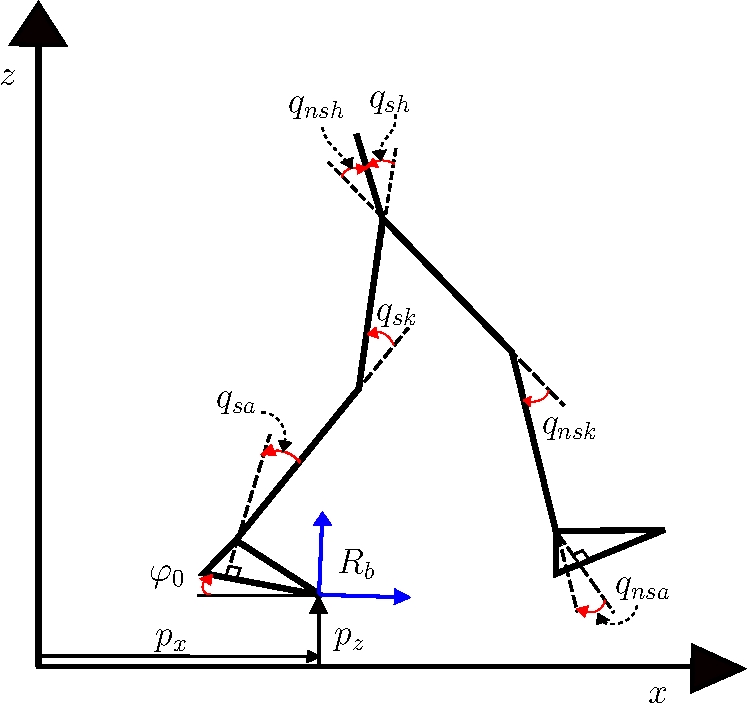
\includegraphics[width=0.45\textwidth]{figures/RobotCoords.pdf}
\caption{Coordinates of 9-Dof planar bipedal robot. The coordinates $(P_{x},P_{z},\varphi_{0})$ represent the position and orientation of the body fixed frame $R_{0}$ in the world frame.}
\label{fig:robot}
\end{figure}

\newsec{Degrees of Freedom and Actuation. }
Holonomic constraints reduce the number of degrees of freedom of the system. Let $n$ denote the number of generalized coordinates of the unconstrained biped, such that $\ConfigurationSpace \in \Reals^n$. Let $\indexbyrobot{n} = \indexbyrobot{m}$ denote the number of indepedent actuators, e.g. motors, on the robot. Let $n_{\indexbyvertex{\contact}}$ denote the number of independent contact constraints for $\vertex \in \VertexSet$. The robot is said to have a number of degrees of freedom, $\indexbyvertex{n}$ for each $\vertex \in \VertexSet$ given by $\indexbyvertex{n} = n - n_{\indexbyvertex{\contact}}$.
\begin{mydefinition}
The robot is said to have
\begin{itemize}
 \item Full actuation, if  $\indexbyvertex{n} = \indexbyrobot{n}$,
 \item Underactuation, if $\indexbyvertex{n} > \indexbyrobot{n}$,
 \item Overactuation, if  $\indexbyvertex{n} < \indexbyrobot{n}$,
\end{itemize}
\end{mydefinition}
\begin{myexample}
 For AMBER 2, $n=9$ and $\indexbyrobot{n} = 6$. For $v=[sh,nst]= ds$, $n_{c_{ds}}=4$ thus $n_{ds} = n - n_{c_{ds}} = 9 - 4 = 5 < 6$ and the robot is overactuated in $ds$. For $v=[sh,st]= fa$, $n_{c_{fa}}=3$ thus $n_{fa} = n - n_{c_{fa}} = 9 - 3 = 6$ and therefore the robot is said to be fullyactuated in $fa$. For $v=[st]= ua$, $n_{c_{ua}}=2$ thus $n_{ua} = n - n_{c_{ua}} = 9 - 2 = 7>6$ and therefore the robot is said to be underactuated in $ua$. It is useful to refer to this example when reading the control section.
\end{myexample}

\newsec{Domain Breakdowns.} A domain breakdown is a directed cycle together with a specific choice of contact points on every vertex of that graph. To define this formally, we assign to each vertex a binary vector describing which contact points are active in that domain.

\begin{mydefinition}
 Let $\ContactSet = \{ \contact_1, \contact_2, \ldots, \contact_\dimensioncontacts\}$ be a set of contact points and $\cycle = (\VertexSet, \EdgeSet)$ be a cycle. A domain breakdown is a function $\DomainBreakdown: \cycle \to \Integers_2^\dimensioncontacts$ such that $\DomainBreakdown(\vertex)_i = 1$ if $\contact_i$ is in contact on $\vertex$ and $\DomainBreakdown(\vertex)_i=0$ otherwise.
\end{mydefinition}

\begin{myexample}
 In the case of the graph given in Example 1 and a set of contact points $\ContactSet = \{ sh, st, nsh, nst\}$, for the domain breakdown given in Fig. 1, this domain breakdown is formally given by $\DomainBreakdown : \cycle_w \to \Integers_2^4$ where $\DomainBreakdown_w([sh,nst])$, $\DomainBreakdown_w([sh,st])$, $\DomainBreakdown_w([st])$, $\DomainBreakdown_w([sh,nst])$ are given by:
 \begin{align}
  \DomainBreakdown_w(\cycle): \left[
  \begin{array}{c} 1\\ 0\\ 0 \\ 1 \end{array} \right] \to
  \left[
  \begin{array}{c} 1\\ 1\\ 0 \\ 0 \end{array} \right] \to
  \left[
  \begin{array}{c} 0\\ 1\\ 0 \\ 0 \end{array} \right] \to
  \left[
  \begin{array}{c} 1\\ 0\\ 0 \\ 1\end{array} \right]
 \end{align}

\end{myexample}


\subsection{Hybrid Control System for AMBER 2}
We now demonstrate that given a Lagrangian, a directed cycle, and a domain breakdown, a hybrid system can be explicitly constructed. Since the Lagrangian is intrinsic to a robot, this result proves that a domain breakdown, which is determined by the enforced contact points, alone dictates the mathematical model of a biped.

\newsec{Continuous Dynamics.} We explicitly construct the control system $\xdot = \indexbyvertex{f}(\x) + \indexbyvertex{g}(\x) \control$ through the constraints imposed on each domain through the domain breakdown.

For the domain $\vertex \in \VertexSet$, the holonomicconstraints that are imposed on that domain are given by:
\begin{align}
 \indexbyvertex{\holonomic}(\q) = \holonomic(\q)\DomainBreakdown(\vertex),
\end{align}
where the domain breakdown dictates which constraints are enforced. Differentiating the holonomic constraints yields a \textit{kinematic constraint}:
\begin{align}
 \indexbyvertex{\Jacobian}(\q) \dq = 0,
\end{align}
where $\indexbyvertex{\Jacobian}(\q) = \text{RowBasis} (\frac{\partial \indexbyvertex{\holonomic}(\q)}{\partial \q})$ is a basis for the row space of the Jacobian (this removes any redundant constraints so that $\indexbyvertex{\Jacobian}$ has full row rank). The kinematic constraint yields the \textit{constrained dynamics} on the domain:
\begin{align}
 \GeneralizedInertia\ddq + \CoriolisGravity = \TorqueDistribution \control + \indexbyvertex{\Jacobian}(q)^T \indexbyvertex{\ContactWrench}
 \label{eq_eulerlagrangeconstrained}
\end{align}
which enforces the holonomic constraint; here $\GeneralizedInertia$, $\CoriolisGravity$ and $\TorqueDistribution$ are as in \eqref{eq_eulerlagrange} and $\indexbyvertex{\ContactWrench}$ is the \textit{wrench} containing forces and moments expressed in the reference frame $R_\contact$ REFERENCE. To determine the wrench $\indexbyvertex{\ContactWrench}$, we differentiate the kinematic constraint:
\begin{align}
 \indexbyvertex{\Jacobian}(q) \ddq + \frac{\partial \indexbyvertex{\holonomic}(\q)}{\partial \q} \dq = 0,
\end{align}
and combine this equation with \eqref{eq_eulerlagrangeconstrained} to obtain an expression for $\indexbyvertex{\ContactWrench} (\q,\dq,\control)$ which is affine in $\control$. Therefore, for $\x = (\q^T, \dq^T)^T$, \eqref{eq_eulerlagrangeconstrained} yields the affine control system $\xdot = \indexbyvertex{f}(\x) + \indexbyvertex{g} (\x) \control$.

\newsec{Discrete Dynamics.} We now construct the domains, guards and reset maps for a hybrid system using the domain breakdown.

Given a vertex $\vertex \in \VertexSet$, the domain is the set of admissible configurations of the system factoring in both friction and a unilateral constraint. Specifically, from the wrench $\indexbyvertex{\ContactWrench} (\q,\dq,\control)$, one can ensure that the foot does not slip by considering inequalities on the friction which can be stated in the form: $\indexbyvertex{\frictioncoefficient}(q)^T \indexbyvertex{\ContactWrench}(\q,\dq,\control) \geq 0$, with $\indexbyvertex{\frictioncoefficient}$ a matrix of friction parameters and constants defining the geometry of the foot (see REFERENCE for more details). These are coupled with the unilateral constraint on this domain, $\indexbyvertex{\unilateral}(q) = \unilateral(q) \DomainBreakdown(\vertex)$, to yield the set of admissible configurations:
\begin{align}
\indexbyvertex{\ConstraintMatrix}(\q,\dq,\control) &= \left[
  \begin{array}{c}
    \indexbyvertex{\frictioncoefficient}(q)^T \indexbyvertex{\ContactWrench}(\q,\dq,\control) \\
    \indexbyvertex{\unilateral}(q)
  \end{array}
  \right] \geq 0.
\end{align}
The domain is thus given by:
\begin{align}
 \indexbyvertex{\domain} = \{ (\q,\dq,\control) \in TQ \times \Reals^{\indexbyvertex{\dimensionu}} : \indexbyvertex{\ConstraintMatrix}(\q,\dq,\control) \geq 0 \}.
\end{align}
The guard is just the boundary of this domain with the additional assumption that the set of admissible configurations is decreasing, i.e. the vector field is pointed outside of the domain, or for an edge $\edge =(\vertex, \vertex') \in \EdgeSet$,
\begin{align}
 \indexbyedge{\guard} = \{ (\q,\dq,\control) \in TQ \times \Reals^{\indexbyvertex{\dimensionu}} : \indexbyvertex{\ConstraintMatrix}(\q,\dq,\control) = 0 \hspace{1mm} \\
  \nonumber \text{and} \hspace{1mm} \indexbyvertex{\dot \ConstraintMatrix}(\q,\dq,\control) < 0\}.
\end{align}
The impact equations are given by considering the constraints enforced on the subsequent domain. For an edge $\edge = (\vertex, \vertex') \in \EdgeSet$, the post-impact velocity $\dq^+$ is given in terms of the pre-impact velocity $\dq^-$ by:
\begin{align}
 \dq^+ = \indexbyedge{P}(\q, \dq^-) = (I - \GeneralizedInertia^{-1} \Jacobian_{\vertex'}^T (\Jacobian_{\vertex'} \GeneralizedInertia^{-1} \Jacobian_{\vertex'}^T)^{-1} \Jacobian_{\vertex'}) \dq^-
\end{align}
with $I$ the identity matrix. This yields the reset map:
\begin{align}
 \indexbyedge{\resetmap}(\q,\dq) = \left[
    \begin{array}{c}
      \q \\
      \indexbyedge{P}(\q,\dq)
    \end{array}
    \right]
\end{align}
The end result is that given a domain breakdown and a bipedal robot, the hybrid model for the biped is completely determined.









